% Principally, this chapter should describe the work which was undertaken before code was written, hardware built
% or theories worked on. It should show how the project proposal was further refined and clarified, so that the
% Implementation stage could go smoothly rather than by trial and error.

% Throughout this chapter and indeed the whole dissertation, it is essential to demonstrate that a proper 
% professional approach was employed.

% The nature of this chapter will vary greatly from one dissertation to another but, underlining the professional 
% approach, this chapter will very likely include a section headed “Requirements Analysis” and incorporate other 
% references to software engineering techniques.

% The chapter will cite any new programming languages and systems which had to be learnt and will mention 
% complicated theories or algorithms which required understanding.

% It is essential to declare the Starting Point (see Section 7). This states any existing codebase or materials 
% that your project builds on. The text here can commonly be identical to the text in your proposal, but it may 
% enlarge on it or report variations. For instance, the true starting point may have turned out to be different 
% from that declared in the proposal and such discrepancies must be explained.

% ~2500 words

\documentclass[final,dissertation.tex]{subfiles}
\begin{document}

\chapter{Preparation}

This chapter begins by providing a high-level overview of how Loopix is structured, a background into some of the cryptography, and details about the development environment and software engineering techniques used.

\section{Structure of Loopix}

In this section, I describe the Loopix network architecture and the Poisson Mix theory. An overview of the network architecture is shown in Figure~\ref{fig:loopix_network}. 

\subsection{Network Architecture}

\begin{figure}[h]
	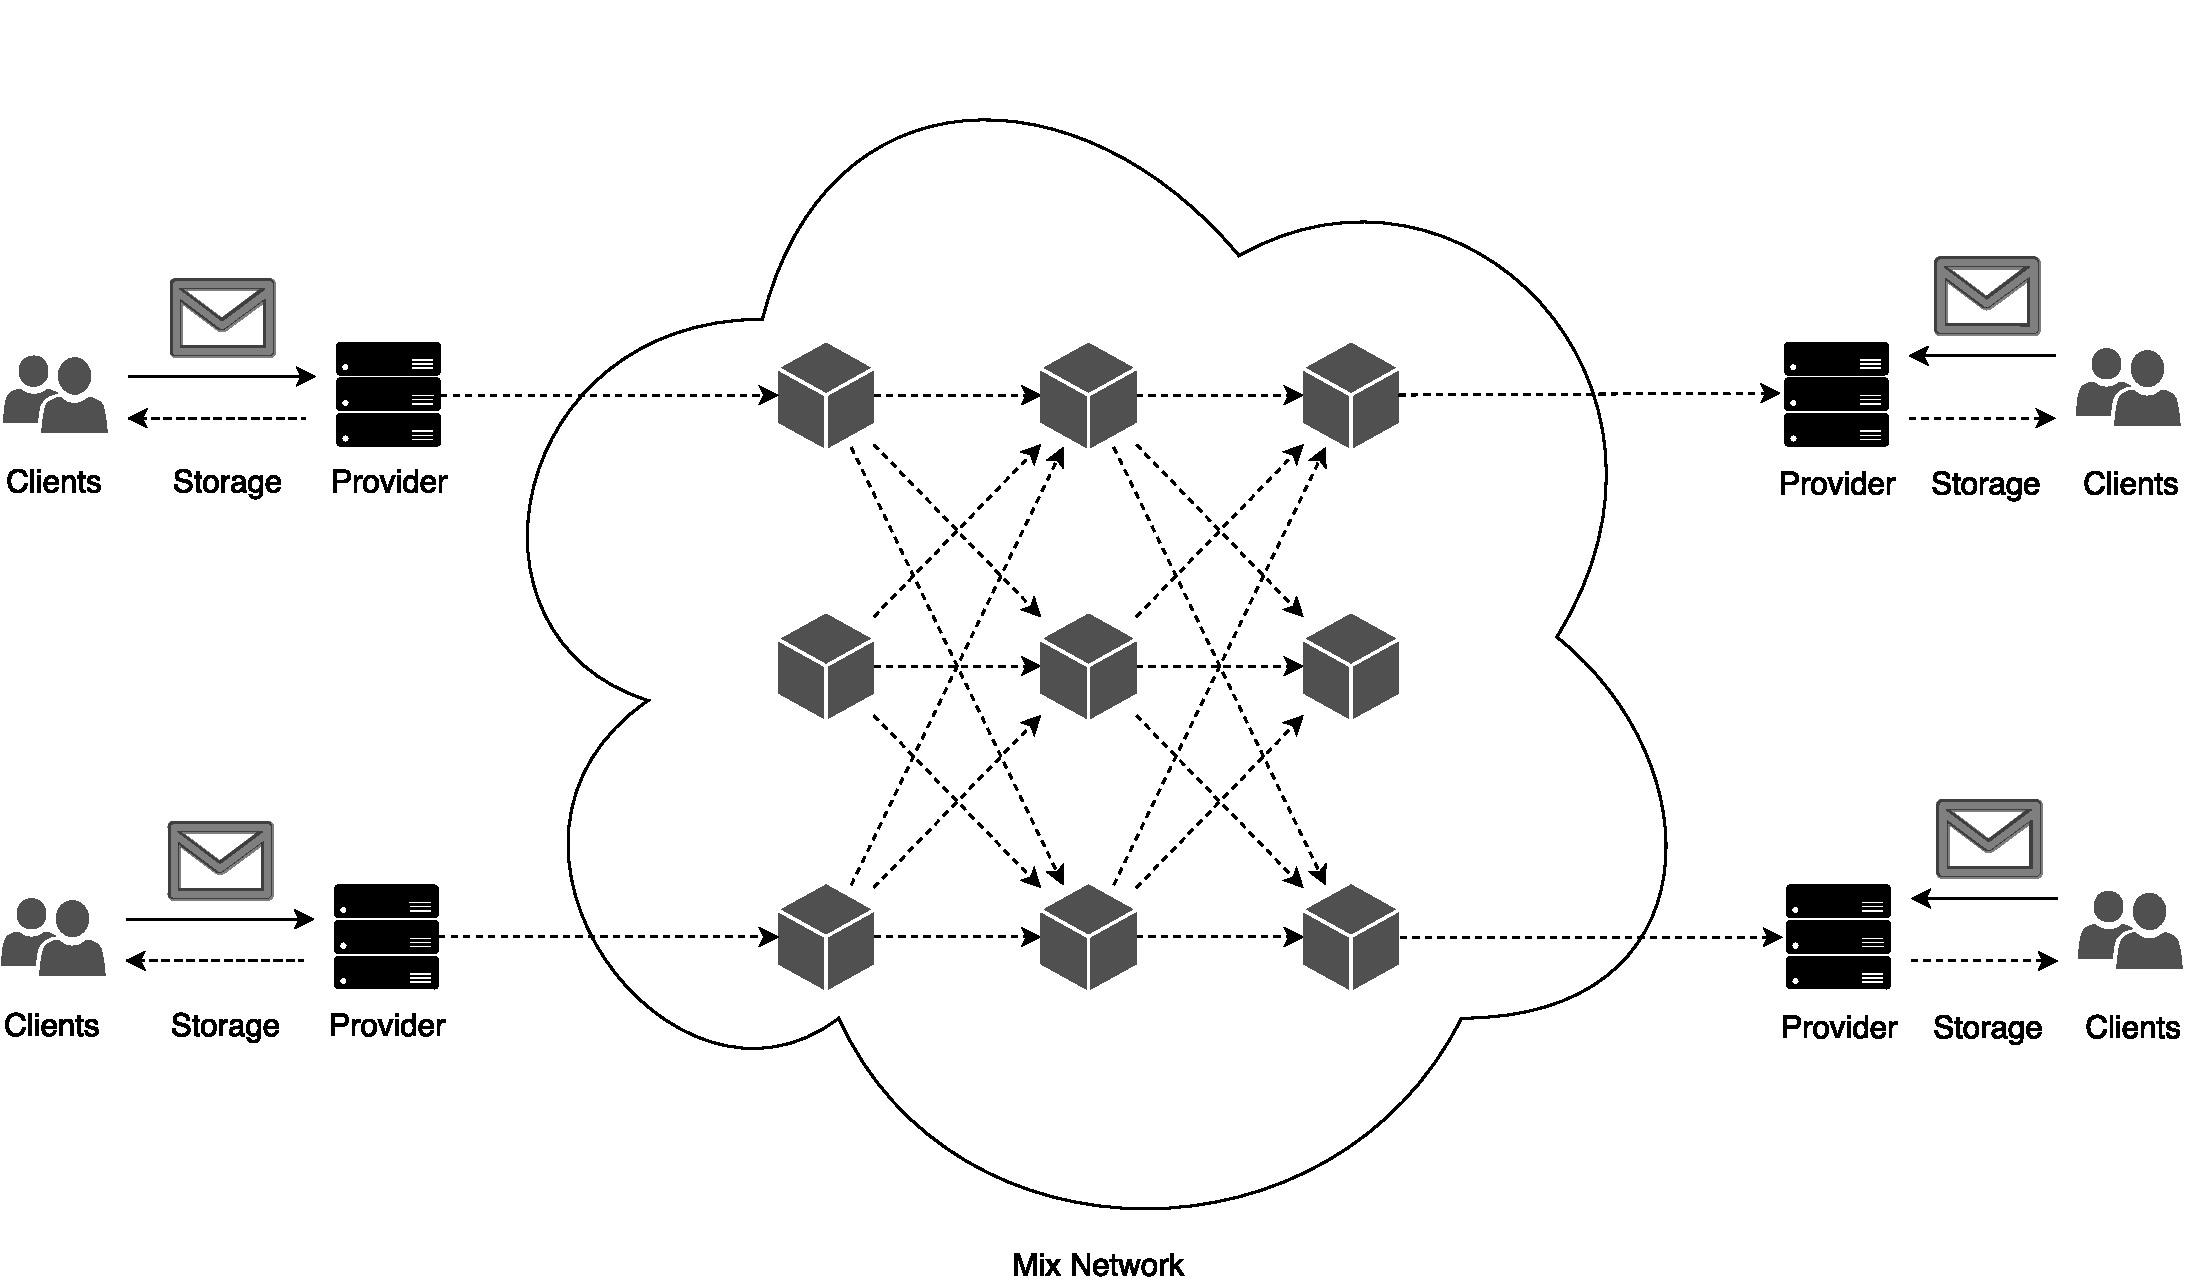
\includegraphics[width=\linewidth]{../figs/loopix_network}
	\caption{Overview of the Loopix network architecture. Clients pass messages to their providers, which are responsible for injecting the message into the mix network. The received messages are stored in inboxes at providers and retrieved by clients when they come online.}\label{fig:loopix_network}
\end{figure}

The Loopix network is composed of three parts: clients, mix nodes and providers. A client can communicate through the Loopix network and can act as a sender and receiver of messages. Each entity in the Loopix network has a unique public-private key pair that is used to encrypt and decrypt messages. The mix nodes are separated into layers, with each layer forwarding messages to the next layer. 

For a sender to send a message to a receiver, the sender needs to know the receiver's Loopix network location, that is the IP address of the receiver's provider, an identifier of the user, and the receiver's public encryption key. The sender also needs to know the network locations of intermediate mix nodes as the sender is responsible for selecting the route through the network.

\subsection{Poisson Mix}

Loopix employs a strategy called the Poisson Mix to prevent observers from learning the correspondences between incoming and outgoing messages at a node, therefore guarding against a global passive adversary performing traffic analysis attacks. 

When a mix packet arrives at a mix node, the mix node decodes and extracts the subsequent mix packet to forward on. The decoded message includes a delay parameter which specifies how long to delay the forwarding of the packet. The source of the message determines the delay parameter. Honest clients choose this delay by sampling from an exponential distribution with a parameter $\lambda$ that is assumed to be public and the same for all mix nodes.

Since honest nodes generate cover traffic, loop traffic, and real traffic following a Poisson process, aggregating these traffic streams at the input of a mix node produces another Poisson process with a rate $\lambda_m$ dependent on the number of mix nodes and clients.

As this input process is a Poisson process, and each message is independently delayed using an exponential distribution with parameter $\lambda$, a Poisson Mix can be modelled as an $M/M/\infty$ queueing system since both input and output of the mix node are Poisson processes. As a result of the memoryless property of such a system, messages are indistinguishable from each other, since messages are emitted with equal probability regardless of the amount of time they have been waiting in the queue.

\section{Requirements Analysis}

The project requires that an implementation and evaluation of Loopix be produced. Java is chosen as the language of choice for the library, and graph generation will be done with Python. The project can be broken down into four parts:

\begin{itemize}
	\item \textbf{Sphinx library} - The packet format used by Loopix. There was an existing Scala implementation\footnote{https://github.com/ndavison21/ScalaSphinx} created as part of a Part II project, but that implementation was incompatible the Python library.
	\item \textbf{Loopix client} - The client handles communication with the network and generating traffic using the Poisson mix strategy. 
	\item \textbf{Demonstration application} - Any application that uses the client for communication, such as instant messaging or email.
	\item \textbf{Test framework} - A framework for testing my libraries, with respect to functionality and performance.
\end{itemize}

As there is already an implementation of Loopix, and binary compatibility is required, I have to refer to the behaviour of the implementation rather than the paper. This is because the paper does not describe sufficient implementation detail.

The choice of Java is a result of the aim of getting Loopix on Android devices. Java is the primary language used on Android. Android supports running native code such as C++, which would result in a more portable library. However, Java was chosen as a pure-JVM library would be easier to integrate into an Android application.

\section{Cryptography}

\subsection{Elliptic Curves}

Elliptic curve cryptography (ECC) is used in public-key cryptography. ECC is based on elliptic curves groups, which are sets of 2D coordinates $(x, y)$ of the form $y^2 = x^3 + Ax + B$ and an additional point at infinity. The key group operation addition $P_1 + P_2$ is defined as: draw a line through $P_1, P_2$, and the line should intersect the curve at a third point $P_3$. Negate the y coordinate of $P_3$ to get $P_1 + P_2$.

Each curve used in ECC has a base point which is the group generator $G$. Private keys are a random integer $x$, and the corresponding public key is given by 

$$G^x = \underbrace{G + G + \cdots + G}_{x \text{ times}}$$.

It is possible to use ECC to perform Diffie-Hellman key exchange as a result of the associativity of multiplication in a finite field. Loopix uses Ephemeral Elliptic-Curve Diffie-Hellman (ECDHE) key exchange for generating shared secrets. Consider two parties, Alice and Bob. Both Alice and Bob generate a public-private key-pair $PK_A$, $SK_A$ and $PK_B$, $SK_B$ respectively and share their public keys. Bob receive's Alice's public key $PK_A$, which is of the form $PK_A = G^{SK_A}$. Bob generates a shared key by exponentiating Alice's public key with his private key $(G^{SK_A})^{SK_B}$. Alice does the same with Bob's public key $(G^{SK_B})^{SK_A}$. From the associativity of multiplication in a finite field, these two are equal, that is:

$$(G^{SK_A})^{SK_B} = (G^{SK_B})^{SK_A} = G^{SK_A*SK_B}$$

For an attacker to recover $G^{SK_A*SK_B}$ from only $G^{SK_A}$ and $G^{SK_B}$, the two messages that are sent over an unsecure channel and known to adversaries requires solving the computational Diffie-Hellman problem, which is believed to be computationally hard.

With ECDHE, a random key-pair is generated for each communication session instead of using static keys. This provides forward secrecy and prevents attackers from decrypting other communications when a previous key is compromised.

\subsection{LIONESS Wide Block Cipher}

LIONESS is a provably secure wide block cipher \cite{anderson1996two}. It is parametrised with a stream cipher (AES-128-CTR) and a hash function (SHA-256). LIONESS supports arbitrary sized blocks, such that the whole message is treated as a single block. This ensures that any change in the ciphertext would prevent the decryption of the ciphertext. This prevents the tagging of encrypted messages as LIONESS is not homomorphic.

Internally, LIONESS is a four round unbalanced Feistel cipher, the structure of which is shown in Figure~\ref{fig:lioness_feistel}. LIONESS is supposed to take as inputs 4 rounds keys $K_1, K_2, K_3, K_4$, each the length of the hash function output. However, this project uses a variant of LIONESS that takes a single key $K$ and derives from $K$ and the plaintext the required round keys.

\begin{figure}[h]
	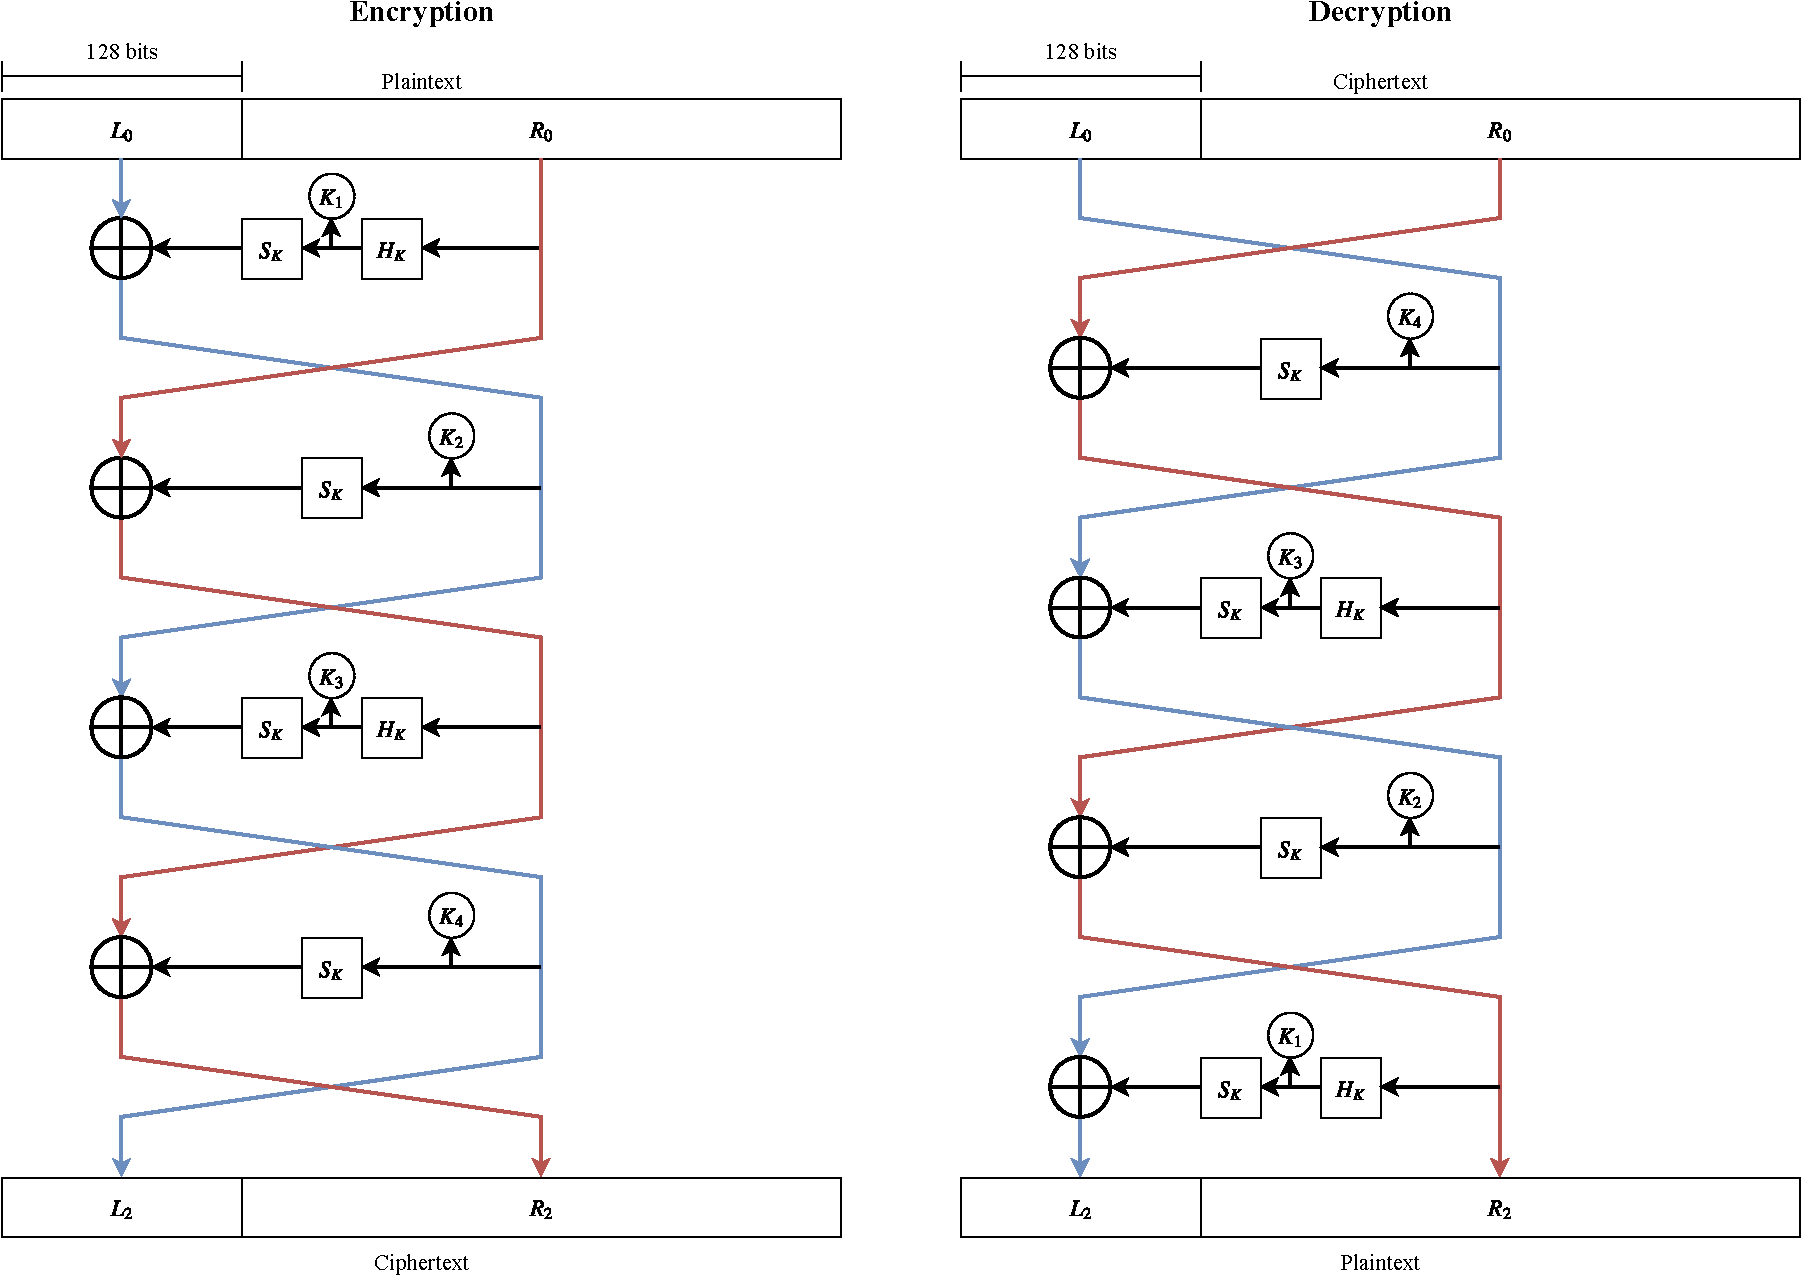
\includegraphics[width=\linewidth]{../figs/lioness_feistel}
	\caption{Feistel network of LIONESS encryption and decryption operations. $S_K$ is a stream cipher keyed using $K$, and $H_K$ is a hash function keyed using $K$.}
	\label{fig:lioness_feistel}
\end{figure}

\section{Development Tools}

A good development environment is essential to productivity. For Java development, the IntelliJ IDEA IDE is used,  with the Gradle build system and JUnit for unit tests. Gradle handles dependency management as well. The Travis CI service is used to run tests on commit to the Git repository. Visual Studio Code is used for writing any Python and shell scripts. Both IDEs provide syntax highlighting, code auto-completion, and code analysis to increase productivity.

Revision control is managed using Git, with remote repositories hosted on GitHub, Bitbucket, and my server to serve as backups. Secondary backups are done by periodically syncing the project repository onto Dropbox and Google Drive.

Docker containers are used to package both Java and Python Loopix applications. Doing this simplifies orchestration of running a test network, and it is simple to swap out a Python client for my client into the network to test. Using Docker containers also simplifies the deployment of the test network on other machines, as I would need to run the tests on a well-equipped server, and containers have dependencies built in that solves many issues.

\section{Existing Libraries}

Many existing libraries are used to avoid reimplementing code that is already available, and some are dependencies as a result of the original implementation using a particular package.

\begin{itemize}
	\item \textbf{Python Loopix and Sphinx libraries} - The existing \verb|loopix| Python package is referenced for implementation details. It is also used for running parts of the test network, such as providers, mix nodes and clients. This package also makes use of the \verb|sphinxmix| package, which is also referenced when implementing my Sphinx library. \verb|loopix| and \verb|sphinxmix| are licensed under the LGPL-3.0 license.
	\item \textbf{Bouncy Castle} - Bouncy Castle is a Java library that provides a cryptography API, with support for various primitives such as AES, SHA, HMAC, and elliptic curves. Bouncy Castle was chosen for easier portability between clients which may not have the official Java cryptography extension installed. Reusing a well-maintained cryptography library is crucial, as implementing my own cryptographic functions properly is difficult, as vulnerabilities such as timing attacks are very easy to introduce. Bouncy Castle is licensed under the MIT license.
	\item \textbf{MessagePack} - MessagePack (\verb|msgpack|) is an efficient binary serialisation format that is extensively used by the Python Loopix and Sphinx libraries. The Java library \verb|msgpack-core| is used for my project. Unlike other serialisation libraries, it does not support serialisation of Plain Old Java Objects, which adds complexity to the usage of the library. \verb|msgpack-core| is licensed under the Apache-2.0 license.
	\item \textbf{Apache MINA} - Apache MINA is an event-driven asynchronous networking library. This is used to simplify working with network sockets since the library handles threading and state management and exposes a simple send and receive interface. MINA is licensed under the Apache-2.0 license.
	\item \textbf{JUnit} - JUnit is a testing library for Java. It is used to support the test-driven development method by allowing the writing and execution of unit tests. JUnit is licensed under the Eclipse Public License.
	\item \textbf{SQLite} - \verb|sqlite-jdbc| is a library for interacting with SQLite databases, which are used in Loopix to hold network information. It is licensed under the Apache-2.0 license.
\end{itemize}

\section{Software Engineering Techniques}

As binary compatibility is important, test-driven development is adopted to ensure my implementation is generating identical output to the Python implementation. This is done by generating test cases using the Python code and using unit tests to compare the output from the Java code. The test cases also include decoding output from the Python implementation. Changes are then made until the tests pass. This also ensures that any changes that causes regressions will be caught by the unit tests.

\end{document}